\documentclass[11pt,a4paper]{article}

\usepackage[margin=2.5cm]{geometry}
\usepackage{graphicx}
\usepackage{booktabs}
\usepackage{caption}
\usepackage{float}
\usepackage{parskip}

\captionsetup{font=small}

\begin{document}

\begin{center}
  {\Large \textbf{Progress Report}}\\[6pt]
  {\large A Multi-Objective Modified Firefly Algorithm for Joint Feature Selection and
  Hyperparameter Optimization of LSTM Networks: An Application to the Colombo Stock Exchange}\\[12pt]
  H.V.A.S. Udayanga (AS2022359)\\
  Department of Computer Science, University of Sri Jayewardenepura\\[4pt]
  29 September 2026
\end{center}

\section{Introduction}

This report explains the work I have done so far, the problems I found while testing,
how I fixed them, and the first results from two baseline methods. I have not run the
MOMFA algorithm on the full experiment yet, so there are no MOMFA results in this report.

\section{Work Completed}

\subsection{Data}
I collected daily price data (open, high, low, close and volume) for the 10 selected CSE
companies (JKH, COMB, DIAL, HNB, LOLC, SAMP, NTB, HHL, DIST, HAYL) from TradingView. The data
is from March 2021 to December 2025. Missing days were filled using the previous day's
values, and the 25 technical indicators in the proposal were calculated for each company.
After removing the first rows where the indicators do not have values yet, each company has
1,252 trading days.

\subsection{Evaluation setup}
The data of each company is divided by date into two parts:
\begin{itemize}
  \item Development period: the first 80\% of the data (1,002 days, March 2021 to
        January 2025). All training and tuning is done using this part only.
  \item Test period: the last 20\% of the data (250 days, January 2025 to December 2025).
        This part is used only once, at the end, to report the final results.
\end{itemize}
Inside the development period, I use walk-forward validation as described in the proposal.
There are five validation windows of 126 trading days each, and the training window grows
after each step. Min-Max scaling is fitted using only the training data of each step. All
models are tested on exactly the same days, even when they use different lookback windows.
For the final result, each model is trained on the development period, the last 126 days of
that period are used for early stopping, and then the model is tested once on the test
period. Figure~\ref{fig:split} shows how the data of HNB is divided.

I also wrote unit tests to make sure that no future data is used during training. These
tests check the scaling, the target values, the validation windows and the test split. All
17 tests pass.

\begin{figure}[H]
  \centering
  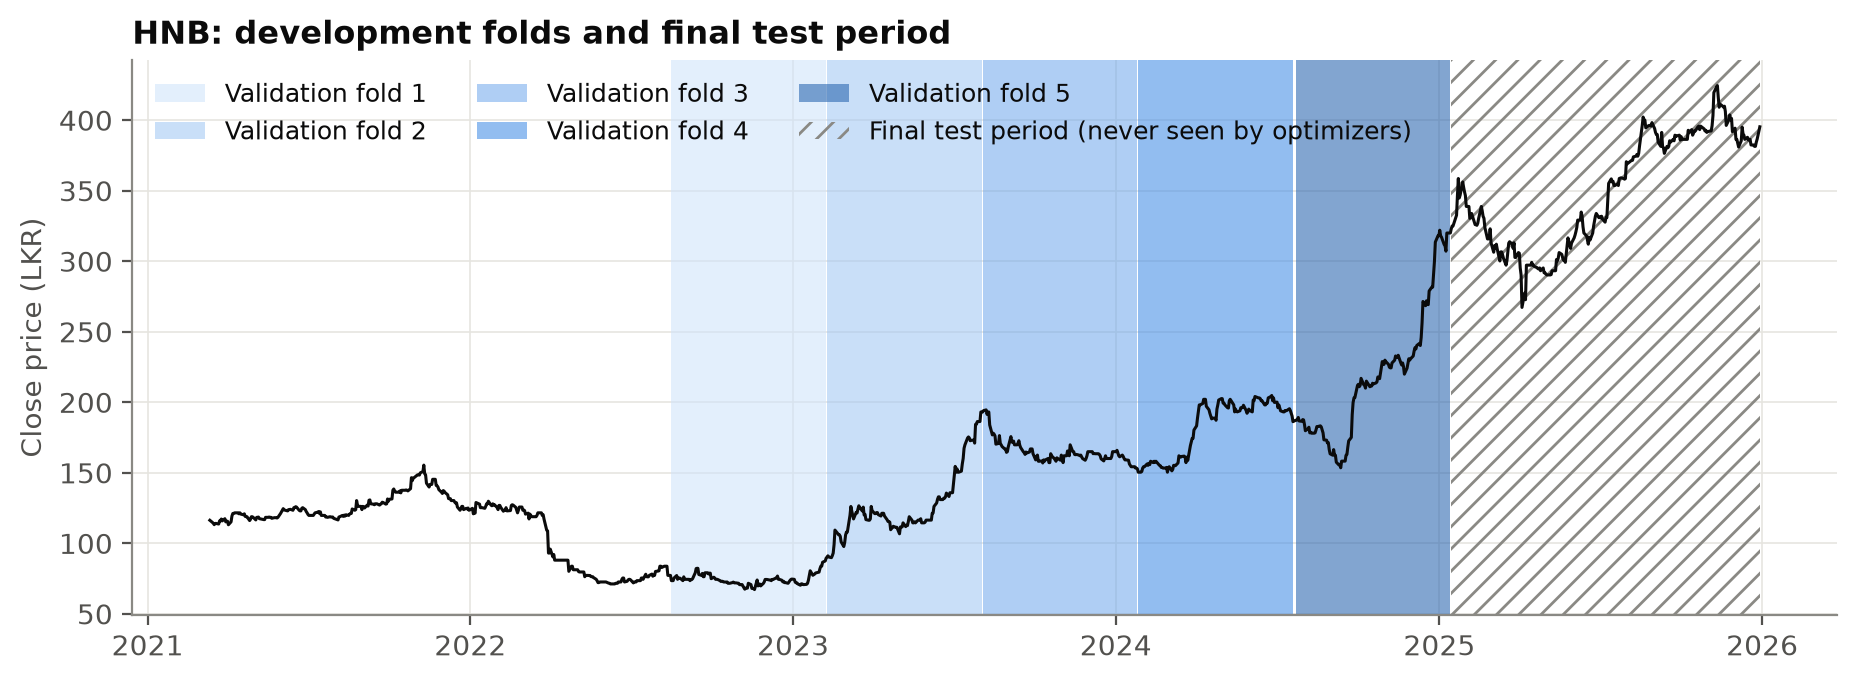
\includegraphics[width=\textwidth]{figures/fold_splits_HNB.png}
  \caption{HNB closing price with the five validation windows and the test period.}
  \label{fig:split}
\end{figure}

\subsection{Models and methods}
\begin{itemize}
  \item The LSTM model and the training settings (maximum 50 epochs, batch size 32, early
        stopping with patience 10, MSE loss) are done. All methods use the same settings.
  \item Random walk baseline: done.
  \item Vanilla LSTM baseline (1 layer, 64 units, learning rate 0.001, dropout 0.2,
        lookback 20, Adam, all 25 indicators): done, with 30 runs for each company.
  \item Grid search baseline (36 settings): code is done and tested, full runs are not
        done yet.
  \item MOMFA parts (solution encoding, Levy flight, sigmoid transfer function, Pareto
        archive): code is done, full runs are not done yet.
\end{itemize}

\section{Problems Found and Changes Made}

\textbf{Predicting the price directly.} In the first version, the LSTM predicted the next
day closing price directly. In the test period, the prices of some companies went much higher
than any price in the training data. For example, the highest HNB price in the training data
was 205 LKR, but in the test period it went up to 424 LKR. The scaler is fitted only on the
training data, so the model was not able to predict such high values. Because of this the
test error was very high (test RMSE of 57.5 for HNB, while the random walk had 5.0).

To fix this, the model now predicts the next day return, which is the percentage change of
the price from today to tomorrow. The predicted price is then calculated as today's closing
price multiplied by (1 + predicted return). All errors are still calculated on the closing
price in LKR, so the aim of the study does not change. After this change, the test RMSE of
HNB came down to 5.9.

\textbf{Other corrections.} I also fixed three smaller problems in the evaluation code. There
was no separate test period, models with different lookback windows were tested on a
different number of days, and the input data was matched with the target of the wrong day
(one day off). All of these were fixed before getting the results below.

\section{First Results}

The four accuracy measures from the proposal are used: RMSE, MAE, MAPE and directional
accuracy (DA). RMSE and MAE are in LKR. MAPE and DA are percentages, so they can be compared
between companies. The random walk simply takes today's price as the prediction for tomorrow,
so it gives the same result every time. Vanilla LSTM values are the average of 30 runs, with
the standard deviation after the $\pm$ sign.

\begin{table}[H]
  \centering
  \caption{RMSE and MAE on the test period (LKR). Lower is better.}
  \label{tab:results_lkr}
  \begin{tabular}{lrrrr}
    \toprule
            & \multicolumn{2}{c}{RMSE (LKR)} & \multicolumn{2}{c}{MAE (LKR)} \\
    \cmidrule(lr){2-3} \cmidrule(lr){4-5}
    Company & Random walk & Vanilla LSTM & Random walk & Vanilla LSTM \\
    \midrule
    JKH  & 0.28 & 0.29 $\pm$ 0.01  & 0.21 & 0.22 $\pm$ 0.01 \\
    COMB & 2.33 & 2.69 $\pm$ 0.28  & 1.45 & 1.87 $\pm$ 0.30 \\
    DIAL & 0.32 & 0.56 $\pm$ 0.16  & 0.21 & 0.41 $\pm$ 0.13 \\
    HNB  & 5.00 & 5.88 $\pm$ 0.65  & 3.30 & 4.32 $\pm$ 0.69 \\
    LOLC & 9.10 & 10.02 $\pm$ 0.40 & 5.85 & 7.19 $\pm$ 0.43 \\
    SAMP & 1.77 & 1.84 $\pm$ 0.09  & 1.17 & 1.29 $\pm$ 0.10 \\
    NTB  & 3.70 & 4.07 $\pm$ 0.42  & 2.32 & 2.76 $\pm$ 0.36 \\
    HHL  & 0.43 & 0.47 $\pm$ 0.05  & 0.29 & 0.35 $\pm$ 0.05 \\
    DIST & 0.96 & 0.99 $\pm$ 0.03  & 0.57 & 0.62 $\pm$ 0.05 \\
    HAYL & 2.63 & 3.94 $\pm$ 0.92  & 1.77 & 3.17 $\pm$ 0.85 \\
    \bottomrule
  \end{tabular}
\end{table}

\begin{table}[H]
  \centering
  \caption{MAPE and directional accuracy on the test period (\%). Lower MAPE and higher
           directional accuracy are better.}
  \label{tab:results_pct}
  \begin{tabular}{lrrrr}
    \toprule
            & \multicolumn{2}{c}{MAPE (\%)} & \multicolumn{2}{c}{Directional accuracy (\%)} \\
    \cmidrule(lr){2-3} \cmidrule(lr){4-5}
    Company & Random walk & Vanilla LSTM & Random walk & Vanilla LSTM \\
    \midrule
    JKH  & 0.93 & 0.99 $\pm$ 0.05 & 22.5 & 40.0 $\pm$ 4.8 \\
    COMB & 0.90 & 1.13 $\pm$ 0.16 & 17.3 & 40.1 $\pm$ 2.6 \\
    DIAL & 1.03 & 1.83 $\pm$ 0.51 & 26.5 & 30.4 $\pm$ 4.1 \\
    HNB  & 0.97 & 1.24 $\pm$ 0.19 & 12.0 & 43.4 $\pm$ 1.3 \\
    LOLC & 0.98 & 1.22 $\pm$ 0.08 & 14.1 & 41.5 $\pm$ 2.3 \\
    SAMP & 0.92 & 1.00 $\pm$ 0.07 & 16.1 & 43.7 $\pm$ 2.5 \\
    NTB  & 1.00 & 1.17 $\pm$ 0.13 & 16.1 & 41.9 $\pm$ 2.0 \\
    HHL  & 1.02 & 1.23 $\pm$ 0.17 & 21.3 & 40.3 $\pm$ 1.8 \\
    DIST & 1.20 & 1.32 $\pm$ 0.11 & 17.3 & 42.5 $\pm$ 2.7 \\
    HAYL & 1.12 & 1.89 $\pm$ 0.46 & 16.1 & 39.8 $\pm$ 1.1 \\
    \midrule
    Average & 1.01 & 1.30 & 17.9 & 40.3 \\
    \bottomrule
  \end{tabular}
\end{table}

Figure~\ref{fig:overview} shows all four measures for every company. RMSE and MAE are shown
divided by the random walk value, so that companies with very different prices can be shown
on the same scale. A value above 1.0 means the vanilla LSTM is worse than the random walk.

\begin{figure}[H]
  \centering
  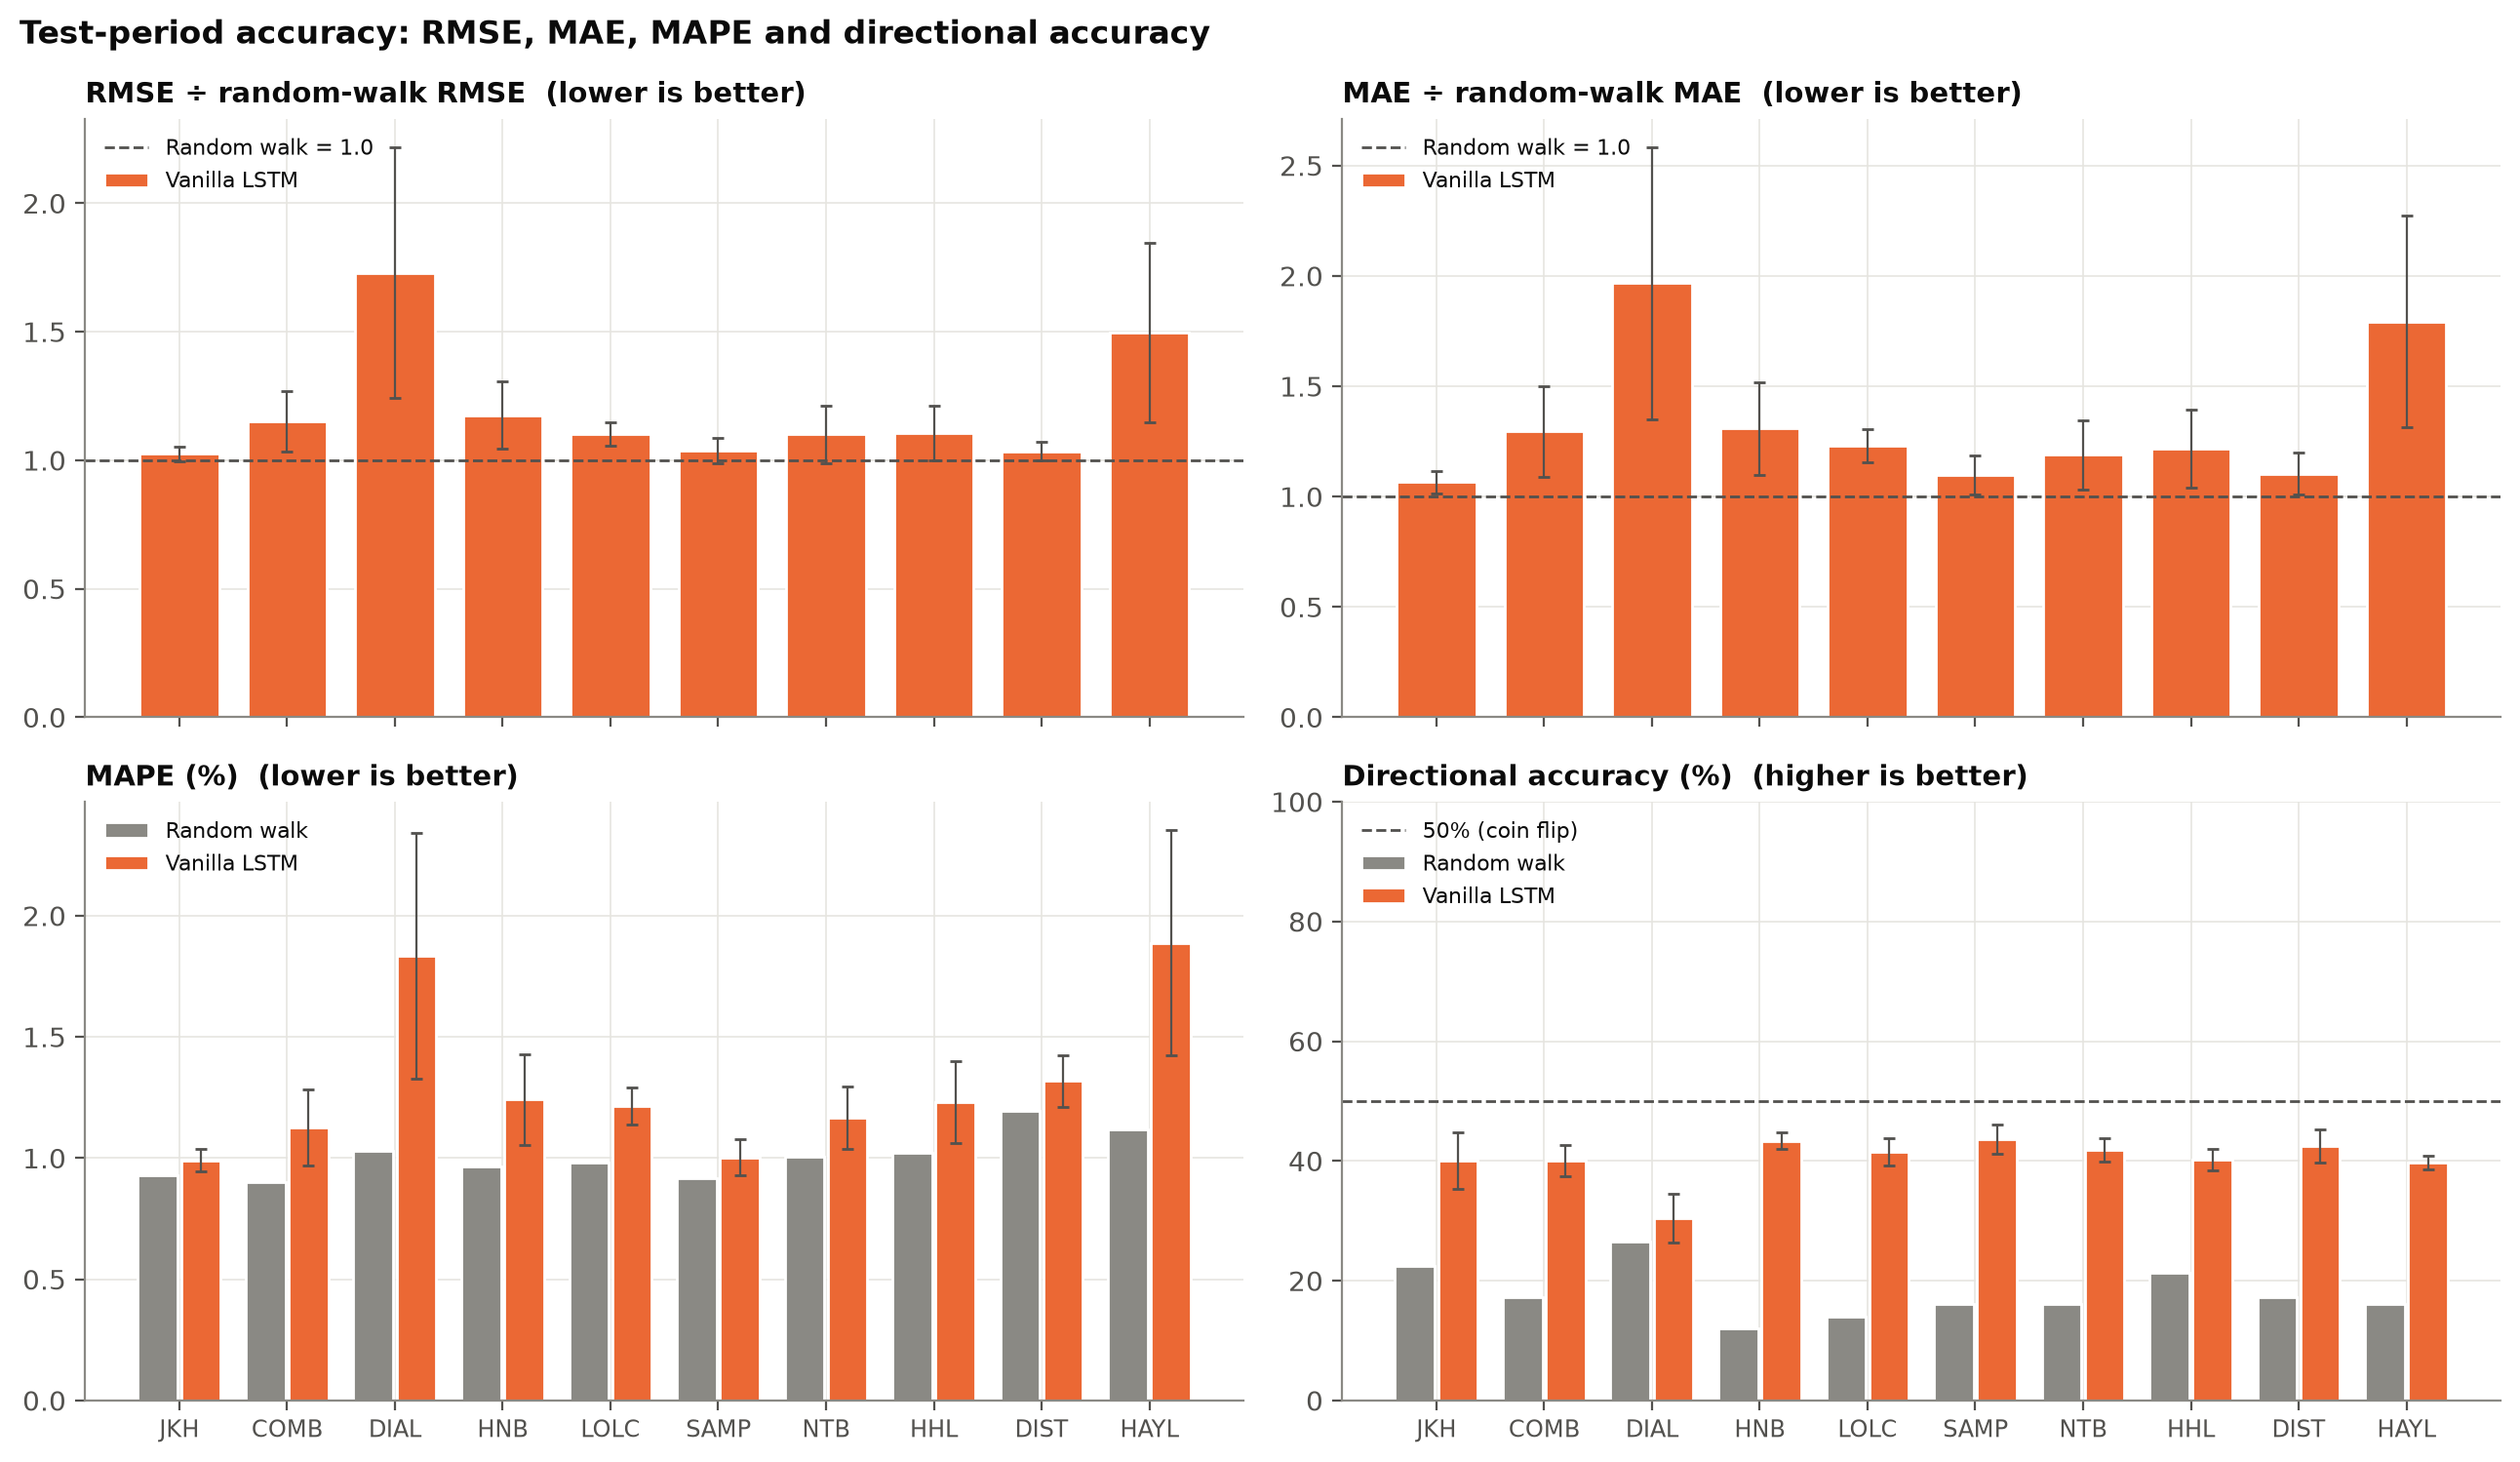
\includegraphics[width=\textwidth]{figures/metric_overview.png}
  \caption{The four accuracy measures on the test period for each company. Error bars show
           the standard deviation over the 30 vanilla LSTM runs.}
  \label{fig:overview}
\end{figure}

What I observed:
\begin{itemize}
  \item The vanilla LSTM is worse than the random walk for all 10 companies on RMSE, MAE and
        MAPE. The difference is small for JKH, SAMP and DIST, and large for DIAL and HAYL. This
        is expected because the vanilla LSTM is not tuned. The important question is whether
        the tuned baselines and MOMFA can do better than the random walk.
  \item Compared with the random walk, the vanilla LSTM does even worse on MAE than on RMSE
        (for example DIAL: RMSE is 1.73 times the random walk, MAE is 1.97 times). This means
        the vanilla LSTM is not only making a few very large errors. Its errors on normal days
        are also bigger than the random walk.
  \item The vanilla LSTM predictions are very close to the previous day's closing price
        (Figure~\ref{fig:pred}). This means the model has mostly learned to repeat the last
        price. I will add a lag check to measure this for all methods.
  \item In the test period most prices were going up, and the vanilla LSTM usually
        predicted a little lower than the actual price.
  \item Directional accuracy is the only measure where the vanilla LSTM is better than the
        random walk (40.3\% against 17.9\% on average). The random walk always predicts no
        change, so it only gets the direction right on days when the price really did not
        change. Both methods are still below 50\%. One reason is that on 12\% to 26\% of the
        test days the price did not change at all, and for the LSTM these days are always
        counted as wrong.
\end{itemize}

\begin{figure}[H]
  \centering
  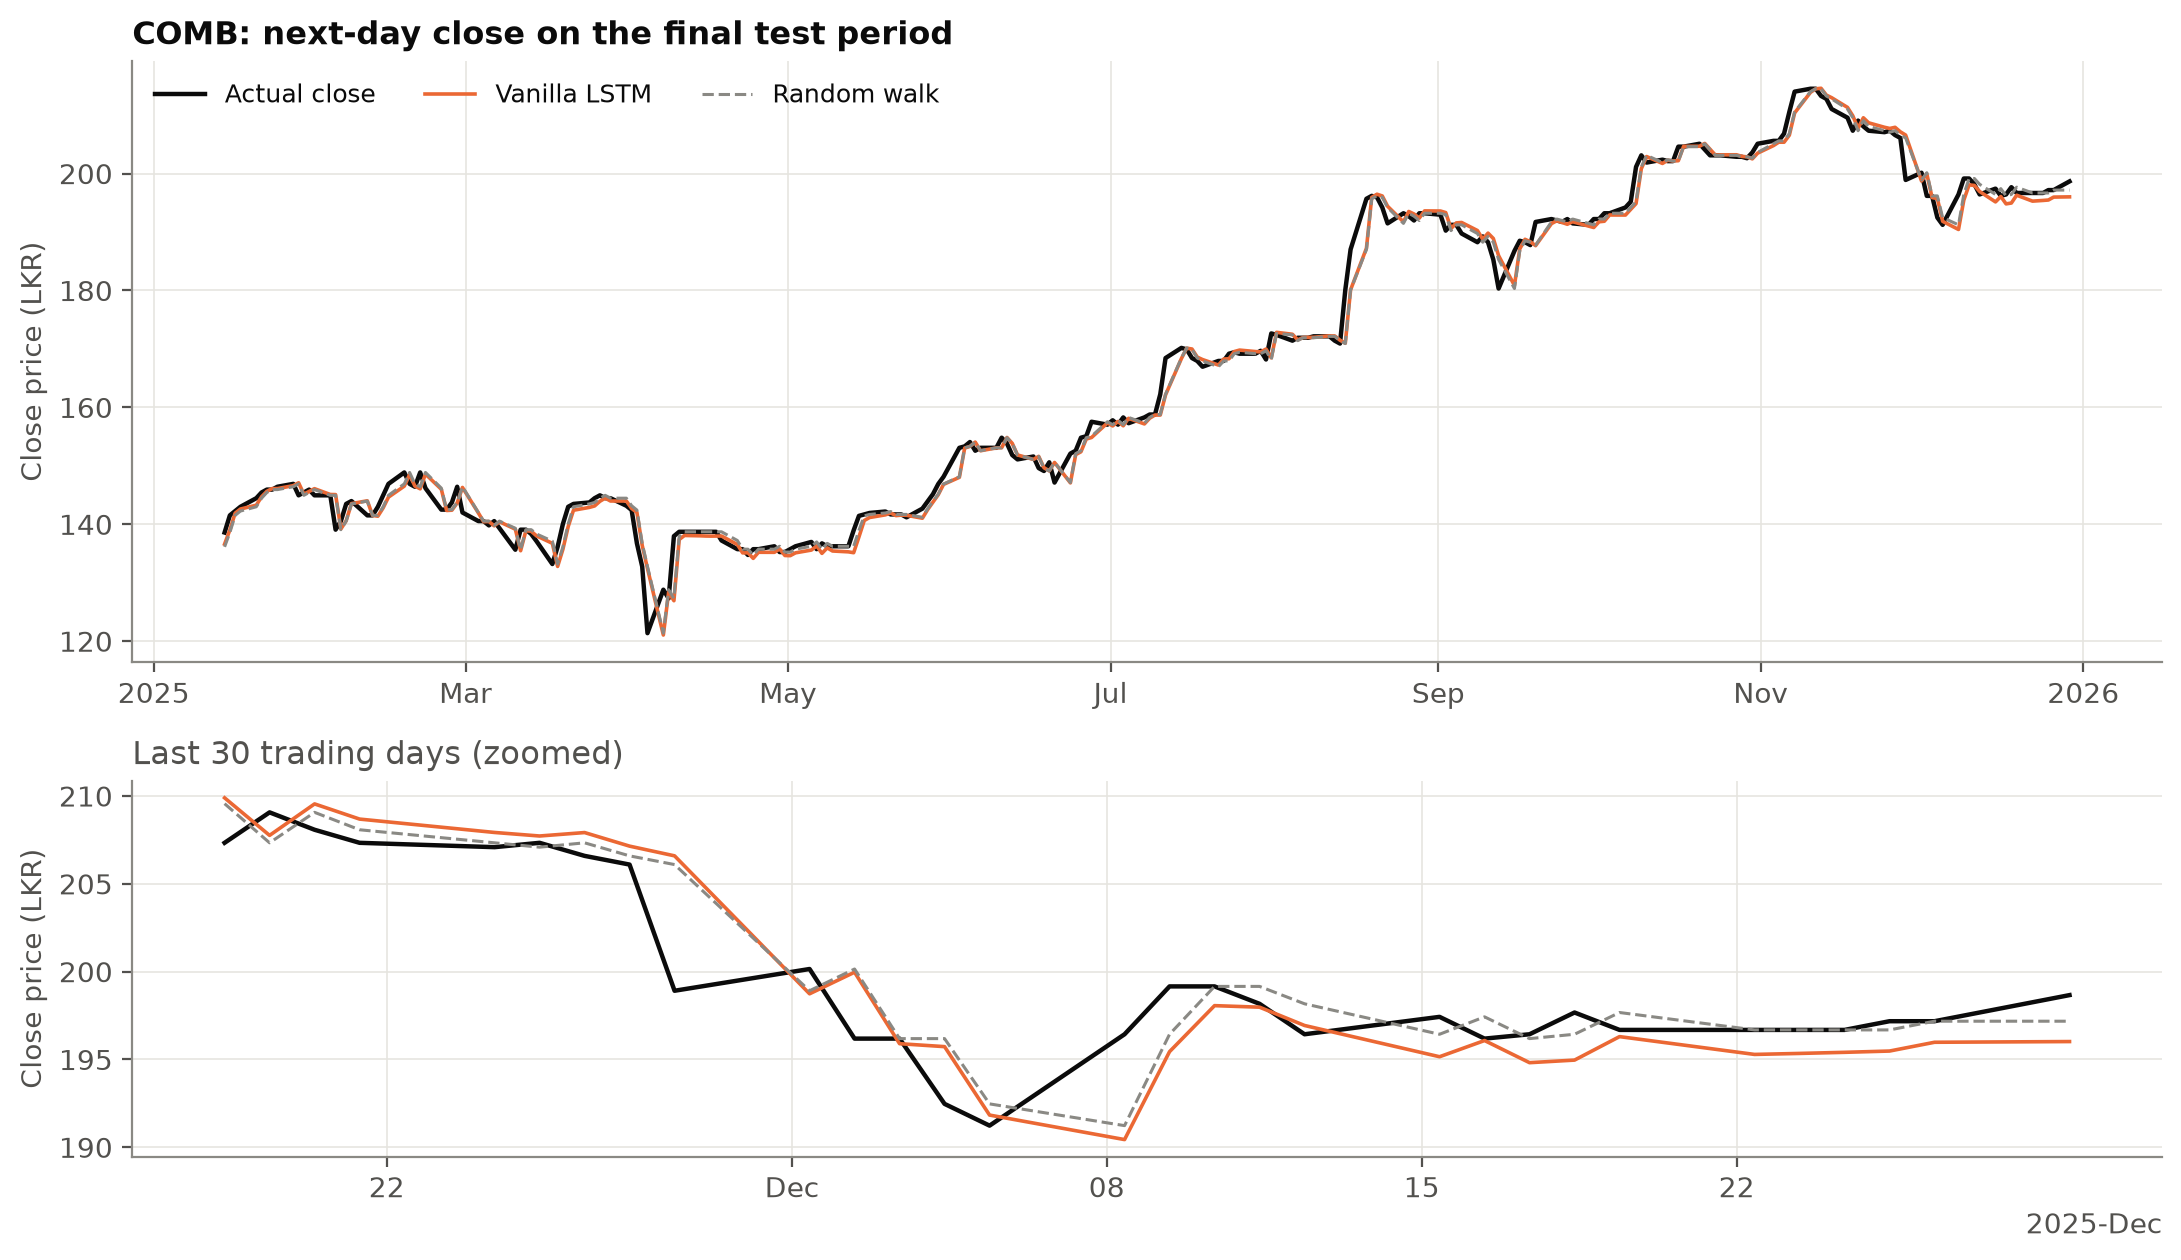
\includegraphics[width=\textwidth]{figures/test_predictions_COMB.png}
  \caption{Actual and predicted closing prices of COMB in the test period. The bottom part
           shows the last 30 trading days.}
  \label{fig:pred}
\end{figure}

\section{Next Steps}

\begin{enumerate}
  \item Run the grid search baseline for all companies.
  \item Write and run the PSO, GA, GWO and WOA baselines.
  \item Run the full MOMFA experiment (30 runs for each company).
  \item Add the Wilcoxon signed-rank tests and the remaining checks (lag check and
        directional accuracy comparison).
  \item Make the Pareto front, hypervolume and feature selection graphs.
\end{enumerate}

\section{Points for Discussion}

\textbf{1. Indicators that are measured in rupees.}
The 25 indicators are of two types. Some indicators always stay inside a fixed range, no
matter what the price is. For example, RSI is always between 0 and 100. Other indicators
are calculated directly from the price, so they are in rupees, the same as the price. These
are the moving averages (EMA9, EMA21, EMA50, SMA20), the Bollinger bands, Parabolic SAR and
VWAP. When the price goes up to a new level, these indicators also go up with it.

This creates the same problem that I found with the target in Section~3, but this time in
the inputs. For HNB, SMA20 was between 70 and 202 LKR in the training data, but went up to
406 LKR in the test period. RSI stayed between 24 and 90 in the test period, which is inside
the range it had in the training data. Since the scaler is fitted only on the training data,
the model gets input values for these indicators that it has never seen before.

There are two options:
\begin{itemize}
  \item Keep the indicators as they are, the same as in the proposal.
  \item Change these indicators so that they are compared with the current price, for
        example SMA20 divided by today's closing price. Then their values stay in a similar
        range even when the price changes a lot. But this changes the feature set given in
        the proposal.
\end{itemize}
I would like to know which option to use before running the full experiments, because this
affects all the methods.

\textbf{2. Days with no price change.}
Directional accuracy checks whether the model correctly says if tomorrow's price will go up
or go down. But on some trading days the closing price does not change at all. This happens
on weekday market holidays (these days are filled with the previous day's price) and on days
when a share is not traded. In the test period, 12\% to 26\% of the days are like this,
depending on the company.

On these days the price did not go up or down, so whatever the model predicts is counted as
wrong. This is one reason why directional accuracy is below 50\% for both methods. I suggest
keeping the definition in the proposal as the main result, and also reporting directional
accuracy using only the days when the price actually changed. This will show how well each
model predicts the direction when the price really moves.

\end{document}
